
\chapter{Robot-Camera Calibration}
\label{chap:robot}
This section presents the theory as well as each individual step for estimating the pose of the camera relative to the robot base frame, the problem to be solved is an extrinsic camera calibration (also known as a robot-camera calibration or Eye-to-hand calibration), but an intrinsic camera calibration needs to be solved a priori. The robot-camera calibration is a fundamental part of the subsequent use in the next chapter of this thesis. The extrinsic camera calibration methods generally require the position of the camera frame relative to a calibration target frame to be known. Therefore, the proposed method to solve the robot-camera calibration task for this thesis is based on tracking a calibration target (standard checkerboard calibration grid) attached to the end-effector of the robot with known forward kinematics. 


\section{Camera Calibration}

Camera calibration is the process of estimating intrinsic and extrinsic parameters. The intrinsic parameters deal with the camera's internal characteristics, such as its focal distance, distortion, and image centre. The extrinsic parameters represent the position and orientation relative to the calibration target. In this thesis the camera calibration is treated separately and can be divided into two main stages:

\begin{itemize}
\item Sensor internal parameter calibration, like lens distortion, focal distance, optical center (image center) described above. In addiction to that, for RGB-D cameras, color and depth image offsets.
\item Robot-camera calibration: the pose(position and orientation) of a camera coordinate system in a reference coordinate frame. In this thesis we also refer as to Eye-to-Hand calibration. The transformation from the camera coordinate system to the robot base coordinates system (also called world coordinates system interchangeably in this thesis) is shown in Figure\ref{fig:system0} 

\end{itemize}
\begin{figure}[!h]
\begin{center}
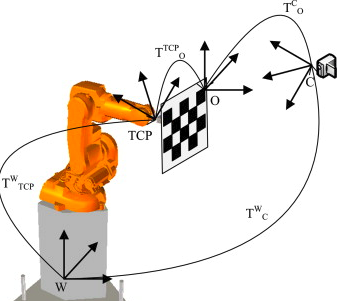
\includegraphics[width=3in]{figures03/system1.png}
\caption{Overview of the camera pose estimation system. The system estimates  the pose of the camera frame relative to the world frame(also known as robot base frame). Image from \cite{autCAL}.}
\label{fig:system0}
\end{center}
\end{figure}

Normally, it is sufficient to perform an internal camera parameter calibration only once for each device unless the lens or sensors itself will be changed or modified. Reliable calibration methods already exist, which are widely used \cite{Zhang} \cite{Tsai}.

Robot-camera calibration, on the other hand, is more application specific and an important stage of any 6-DoF pose estimation system according to \cite{autCAL1} \cite{autCAL2}. 

\section{Sensor internal parameter calibration}

\subsection{Camera Model} \label{intrinsic}

The choice of camera model influences the final calibration results, so the first step is to select an appropriate camera model. In this thesis, the pinhole camera model \ref{pinhole} is used. It describes the mathematical relationship between the coordinates of a point in three-dimensional space and its projection onto the image plane of an ideal camera. 

The MATLAB, Open CV  and the $camera\textunderscore calibration$ ROS  \cite{calRos} packages are the most popular systems for camera calibration. They are already available for checkerboard detection based on the pinhole model and the method proposed by Zhang \cite{Zhang}, All of them introduce the radial distortion and tangential distortion. In this thesis, the OpenCV and $camera\textunderscore calibration$ ROS packages are used for the purpose of comparison in this thesis.
The technique proposed by Zhang only requires the camera to observe a calibration target shown at few (at least three) different orientations. the technique relates known points in the world to points in an image, in order to do so, one must first acquire a series of known world points. The most common method is to use known planar objects(checkerboard calibration grid) at different orientations with respect to the camera to develop an independent series of data points. The calibration object chosen in this thesis is a 6x9 checkerboard with the corner points as the known world points and it can be seen in Figure \ref{fig:target0}.

\begin{figure}[!h]
\begin{center}
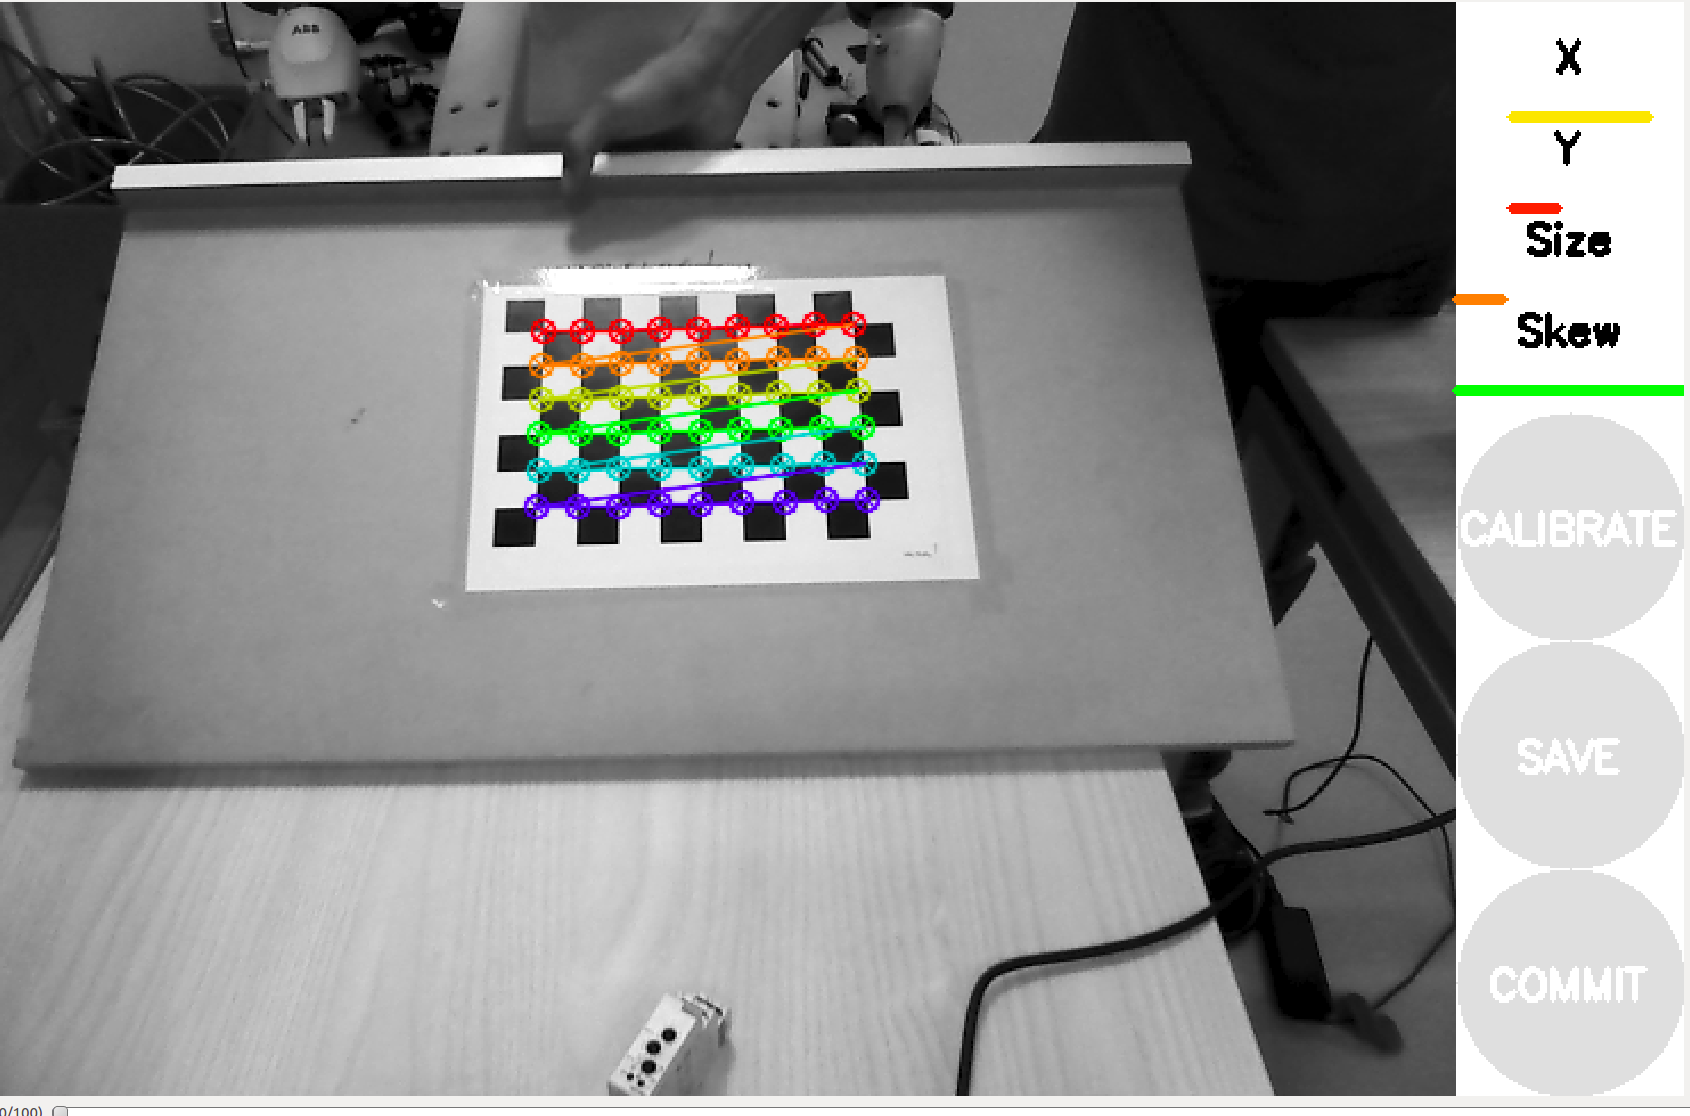
\includegraphics[width=3in]{figures03/intros.png}
\caption{Overview of the intrinsic calibration based on industrial calibration ROS package with a 6X9 checkerboard calibration target}%\cite{temp2}}
\label{fig:target0}
\end{center}
\end{figure}

\section{Eye-to-Hand Calibration}

In order to know the pose of the camera coordinate system relative to the world coordinate system also known as robot base frame, extrinsic calibration (estimation of the rotation and translation of the camera frame) methods will be used. In this thesis, the method for extrinsic camera calibration based on calibration planer target is used. It is assumed camera intrinsic parameters and distortion coefficients are known a priori as describe in \ref{intrinsic} and fixed during the entire sequence. Such a system is shown in Figure \ref{fig:camposest}.


\begin{figure}[!h]
\begin{center}
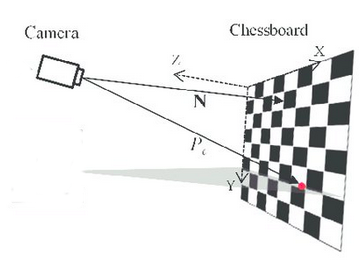
\includegraphics[width=3in]{figures03/camposest.png}
\caption{Overview of the camera pose estimation system. The system estimates the distance
and orientation to the local coordinate system of the checkerboard}%\cite{temp2}}
\label{fig:camposest}
\end{center}
\end{figure}

\subsection{Calibration Targets}\label{caltar}
There are many types of camera calibration targets for use in imaging systems. In this thesis the planar targets are use since they can be easily printed with a standard
printer and fixed to a surface. Planar targets can be subdivided as follow:
\begin{itemize}
\item Repeated pattern e.g. checkerboard patterns 
\item Non repeated pattern e.g augmented Reality (AR)
\end{itemize}

\subsection{Checkerboard Patterns}

Checkerboard calibration targets are one of the most frequently-used targets, where the calibration points are the corner points between squares. This pattern is simple to produce and allows for high accuracy because the corner points can be detected to subpixel precision. For example, the popular OpenCV library already contains algorithms to automatically locate plain checkerboards. Figure \ref{fig:target1} shows an example of checkerboard calibration target.


\begin{figure}[!h]
\begin{center}
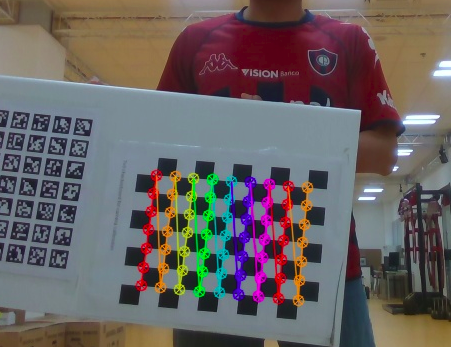
\includegraphics[width=3in]{figures03/openCV1.png}
\caption{Overview of a 7X9 checkerboard calibration grid }%\cite{temp2}}
\label{fig:target1}
\end{center}
\end{figure}

\subsection{Augmented Reality (AR)}
AR markers also called Fiducial (individually identifiable) markers have become increasingly popular in recent years. Such markers can be used in a variety of settings such as camera calibration, where small markers are used, those who encode a unique code for identification purposes. There are a large number of markers available. One of the most common fiducial marker designs includes rectangular patterns with identification codes in the interior such as $ARTag (2005)$, AprilTag and CALTag to name few of them.  Refer to \cite{fiducialTargets} 


\begin{figure}[!h]
\begin{center}
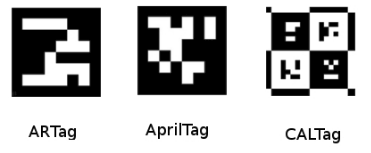
\includegraphics[width=3in]{figures03/fiducials.png}
\caption{ARTag, AprilTag and CALTag markers example. Image from \cite{fiducialTargets}}
\label{fig:fiducial}
\end{center}
\end{figure}

\subsection{Selection}
In this thesis, the checkerboard pattern is used.  This pattern is simple to produce and allows for high accuracy because the corner points can be detected to subpixel precision \cite{planarTargets}. The calibration target located on the custom-made plate is shown in Figure \ref{fig:target2}


\begin{figure}[!h]
\begin{center}
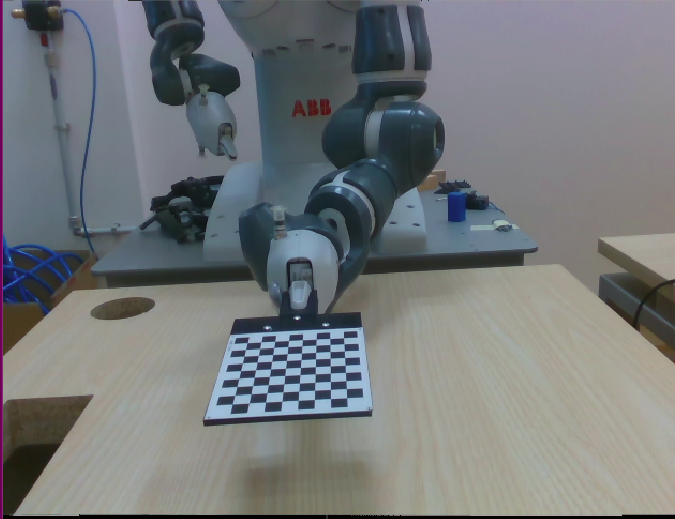
\includegraphics[width=4in]{figures03/target1.png}
\caption{An 8X9 Checkerboard Calibration Target fixed on a custom-made plate}
\label{fig:target2}
\end{center}
\end{figure}

\subsection{Checkerboard Estimator}\label{pose1}

The task of estimating the pose of a calibrated camera given a set of n 3D points in the world and their corresponding 2D projections in the image is a fundamental and well-understood topic in computer vision, and it is referred to as the Perspective-n-Point problem in most of the literature. OpenCV provides solution to solve the Perspective-n-Point problem which return R (rotation) and t(translation).  

A solution to the problem exists for $n = 3$ called P3P, and many solutions are available for the general case of $n\geq 3$. In this thesis, the solution Perspective-n-point(PnP) \cite{pnp} is used, which is already available and well tested in OpenCV a open source communitive. A projection of 3D points expressed in world frame onto the 2D image plane is shown in Figure \ref{fig:target3}.


\begin{figure}[!h]
\begin{center}
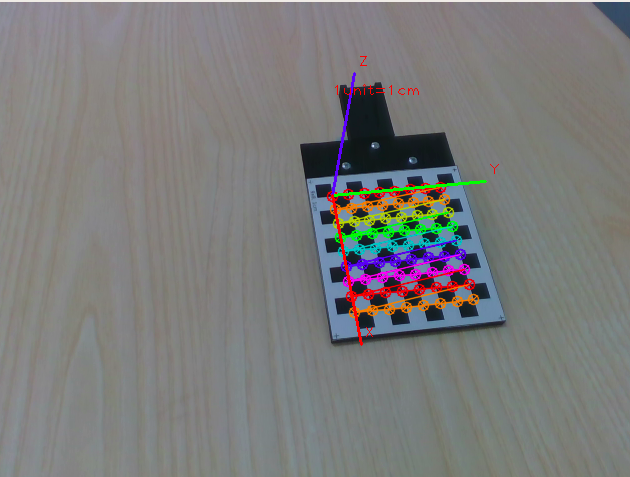
\includegraphics[width=4in]{figures03/calibrationtarget1.png}
\caption{Visualization of the 3D world coordinates system projeted onto the 2D image plane}
\label{fig:target3}
\end{center}
\end{figure}



\subsection{Coordinate Transformation From Robot Base To Camera Frame}
From the rigid transformation theory described in \ref{rigidtf0}, the orientation and translation calculated in \ref{pose1}, can be represented in a 4x4 matrix by employing a homogenous coordinates as follows:

\begin{equation}
\begin{pmatrix}
R & t \\ \label{t}
0 & 1
\end{pmatrix}
\end{equation}

Eq. \ref{t} is called the Euclidean transformation, also known as transform. Where $R \in \mathbb{R}^{3}$ is the rotation matrix and $t \in \mathbb{R}^{3}$ is the translation vector, altogether representing the pose of the camera frame relative to the calibration target frame.\\
It is assumed that the transform between the end-effector(or tool centre point) and the robot base, $ ^{R}T_{TCP}$, is known from the forward kinematics of the robot. In addition to that, the transform from the end-effector frame relative to the calibration target frame, $ ^{TCP}T_{T}$, was defined according to our need when the custom-made plate \ref{fig:target3} was designed.

Since the transform tree is already made, we can retrieve the pose of the camera relative to the robot base frame as follow:

\begin{equation}
^{R}T_{C}= ^{R}T_{TCP} \cdot ^{TCP}T_{T} \cdot ^{T}T_{C}\label{t4}
\end{equation}
In Eq. \ref{t4}, ${R}T_{C}$ represents the transform from the camera frame relative to the robot base frame. Since the whole system is based on the Robot Operative System (ROS) due to its modular design and available integration for a large amount of robot and sensory device, the transform is also retrieved with the help of tf-ROS package. In Figure \ref{fig:tf6}, ${R}T_{C}$ is shown calculated by software mean. 


\begin{figure}[!h]
\begin{center}
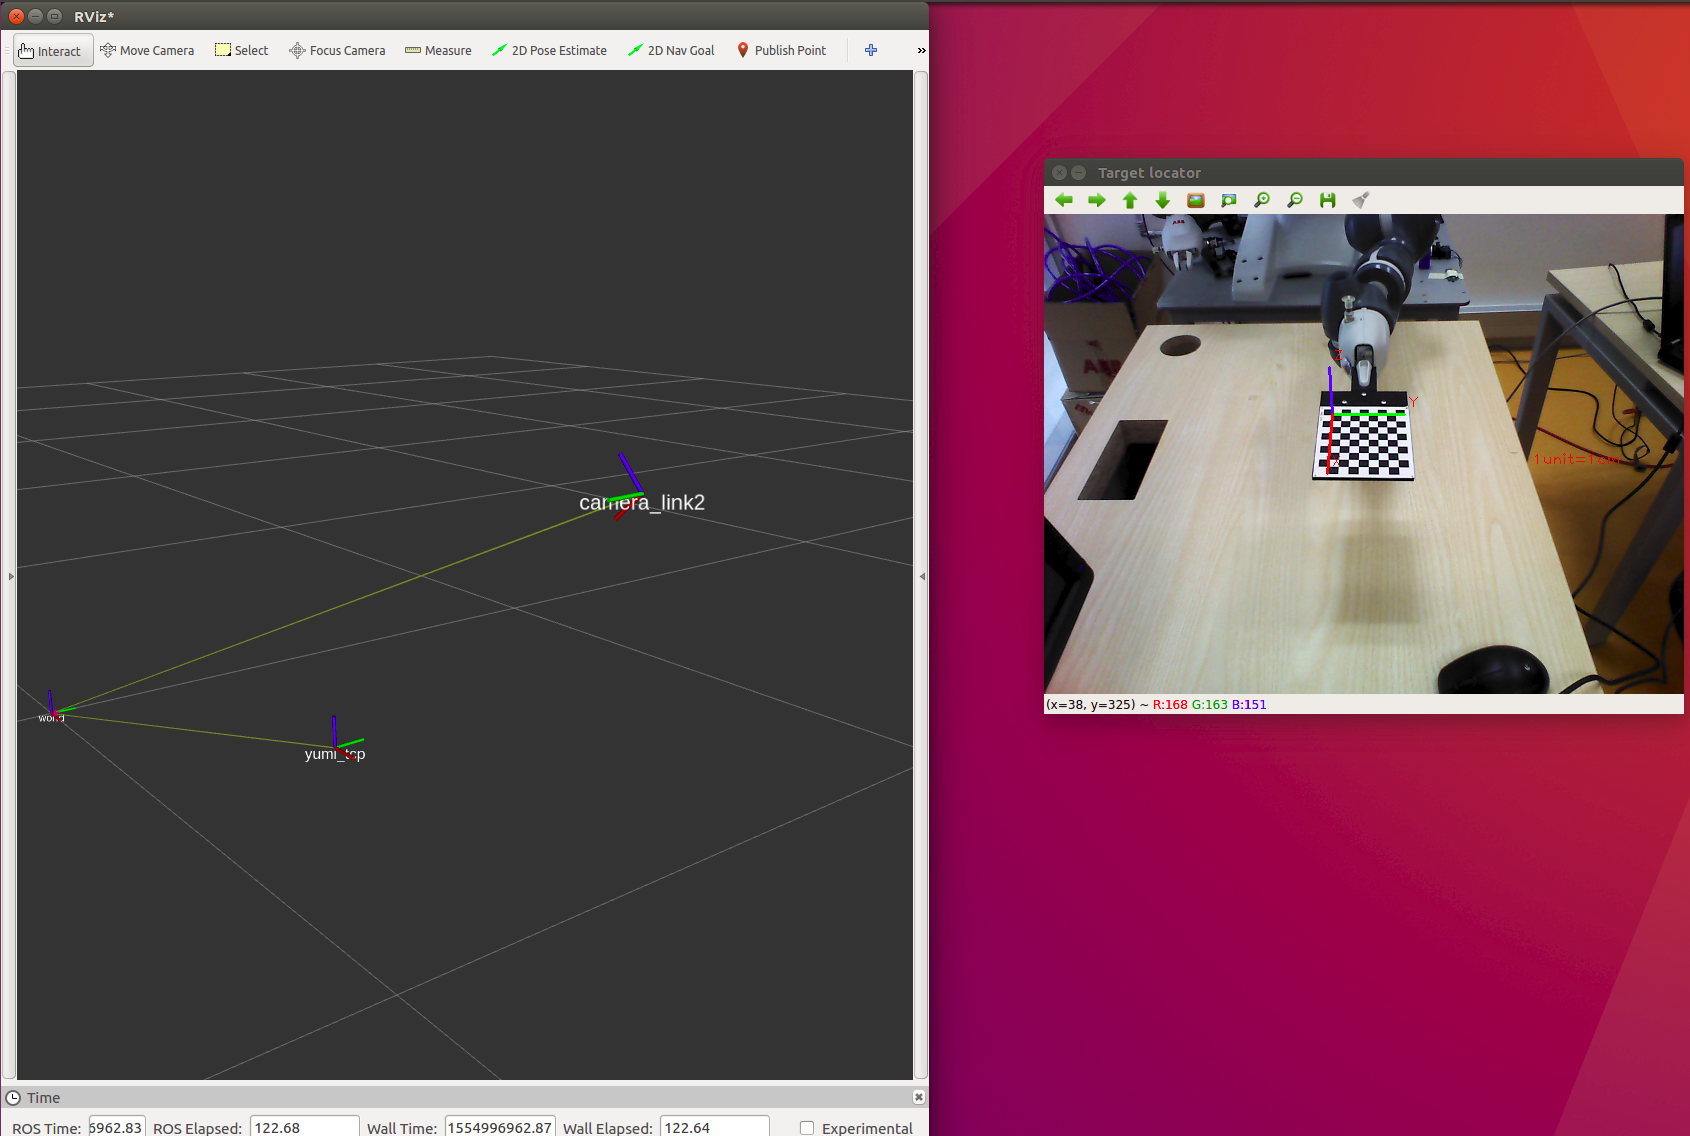
\includegraphics[width=4in]{figures03/rviz1.png}
\caption{Right: Visualization of the transform (camera and target) relative to the robot base frame using ROS Rviz package. Left: Show an image used in the camera pose estimation.}
\label{fig:tf6}
\end{center}
\end{figure}






























